\clearpage
\chapter{Physics Object Definitions}\label{sec:objects}
%reconstruction algorithms, isloation, cleaning, IDs, particle flow

In this section, we provide the definitions of physics objects used in the analysis.

\section{Muons}\label{sec:muons}


The analysis sources the SlimmedMuons collection from the MINIAOD MC datasets to produce {\tt selectedPatMuons}.
Muon objects are required to have 
\begin{itemize}
  \item $pt$ $\geq$ 12 GeV to reach BPH trigger plateau
  \item $|eta|$ $\leq$ 1.5 for L1 seed $|eta|$ cut in BPH trigger
  \item Pass the Loose ID criterion (isLooseMuon) as described in the Muon POG~\cite{muonpog}.
\end{itemize}

\begin{figure}[h!]
  \caption{Data/MC of muon objects}
  \label{fig:muons}
  \centering
  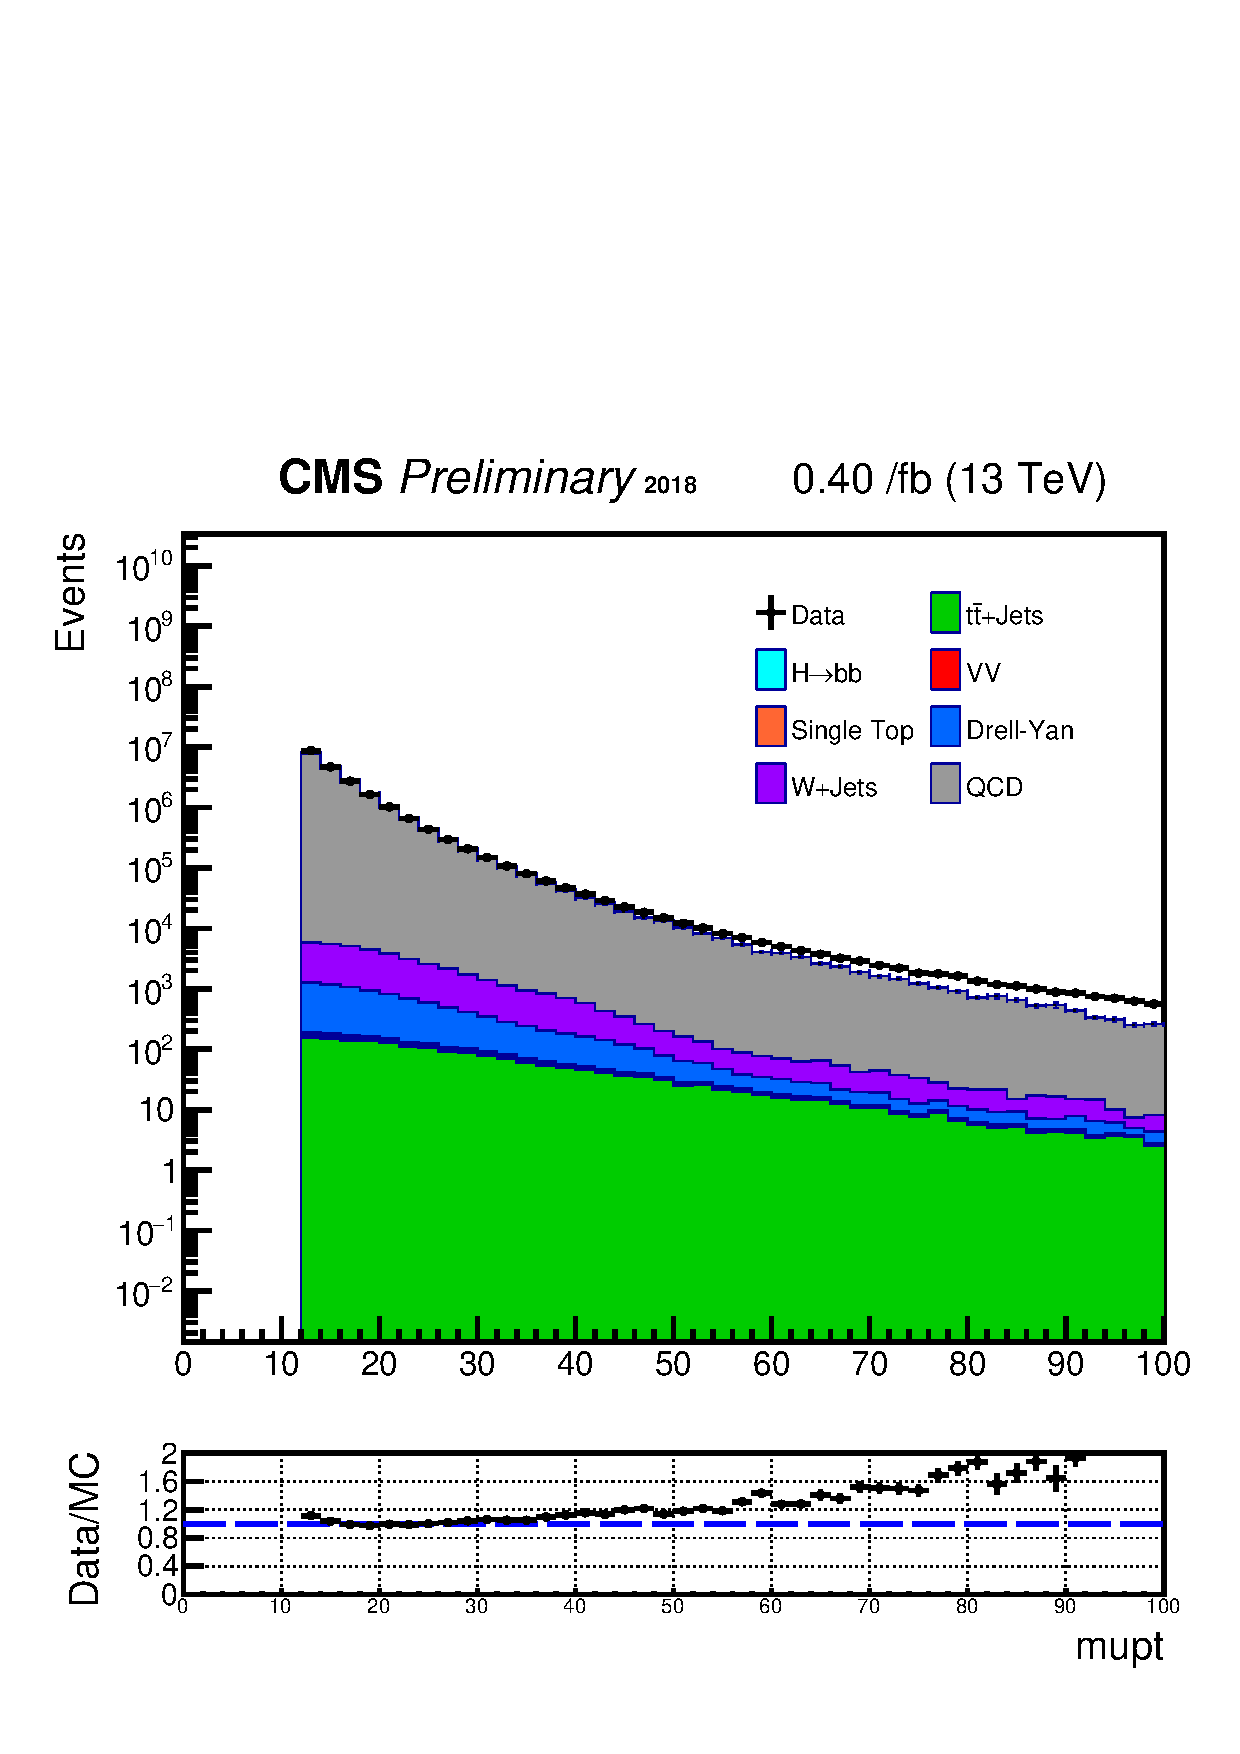
\includegraphics[width=0.47\linewidth]{figs/Data_AnalysisNoteplot_MS-15_ctauS-10_mupt.pdf}
  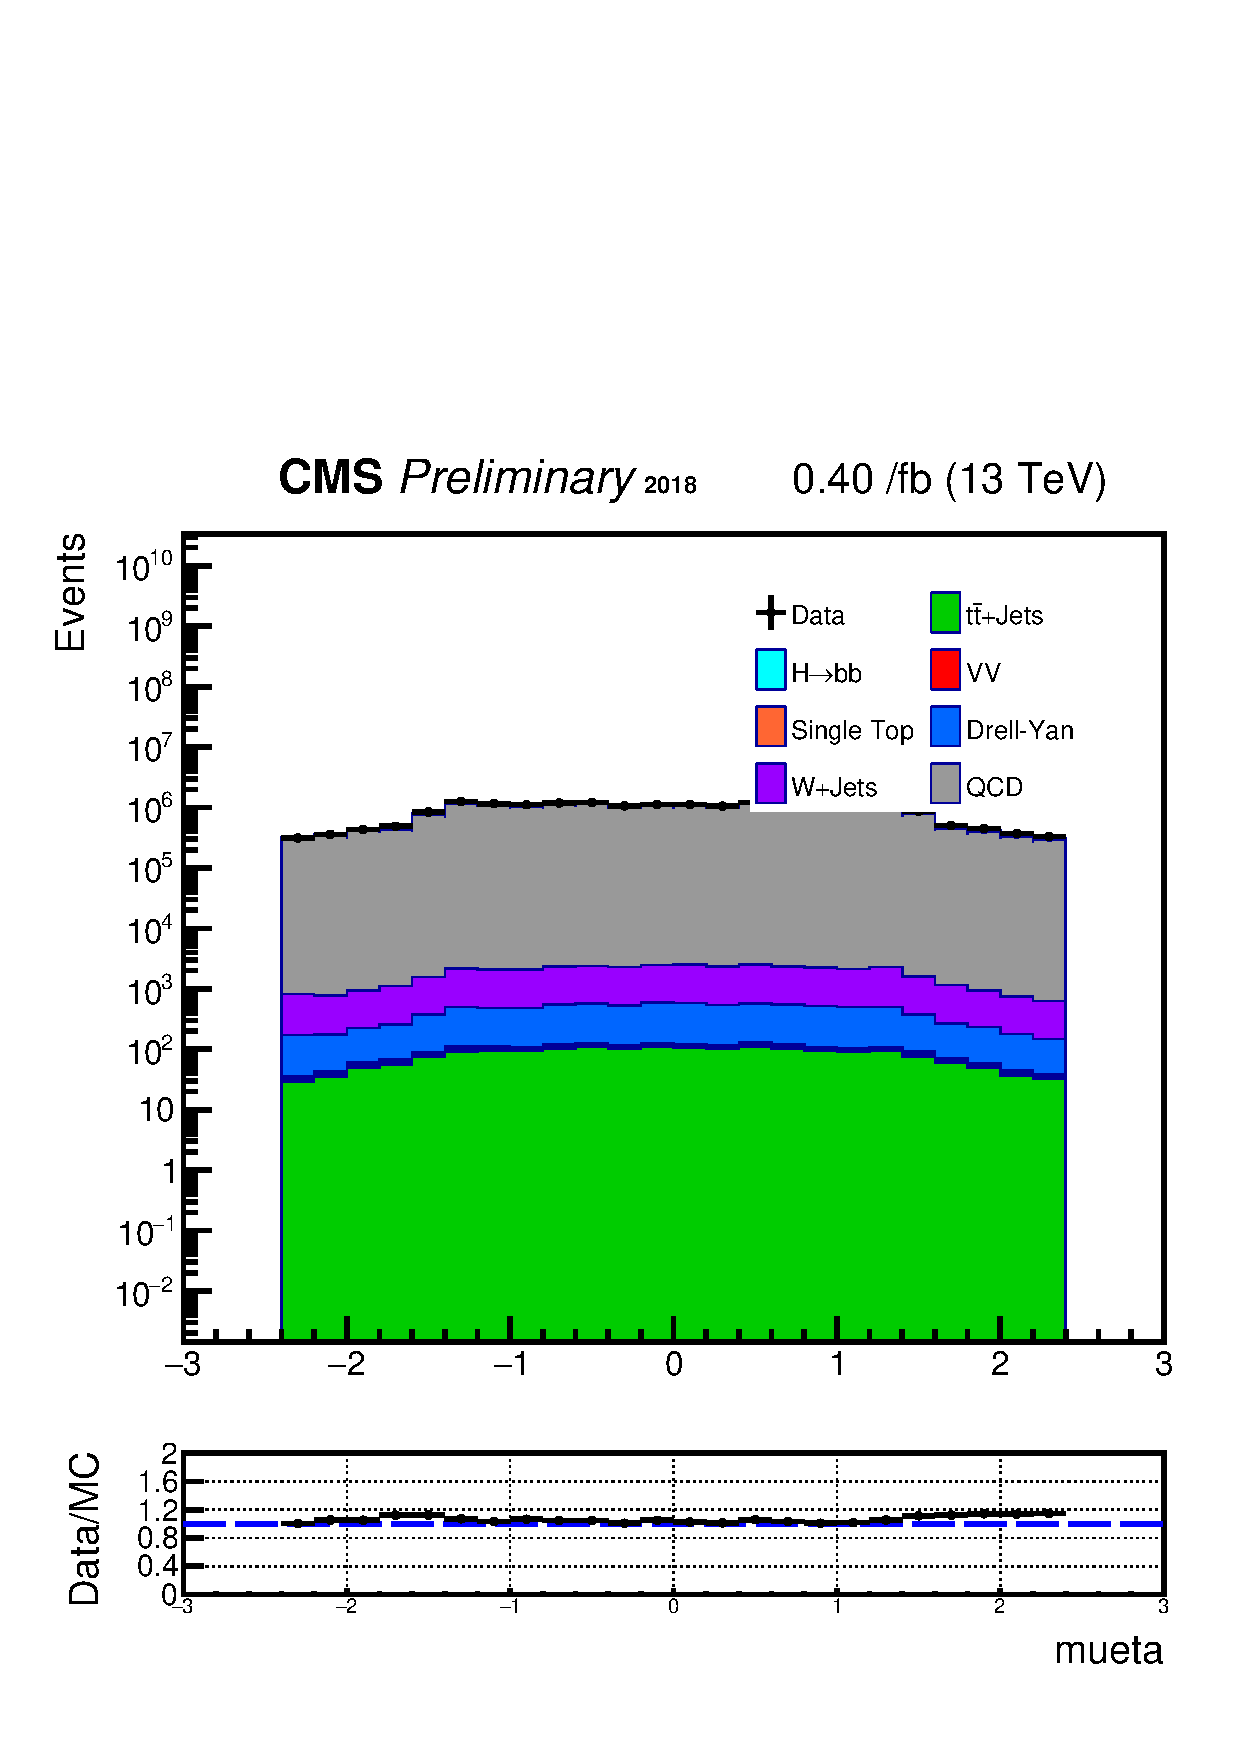
\includegraphics[width=0.47\linewidth]{figs/Data_AnalysisNoteplot_MS-15_ctauS-10_mueta.pdf}
\end{figure}

The motivations for isolation requirements on muons are discussed in Section~\ref{sec:selections}.


\section{Jets}\label{sec:jets}

The analysis sources SlimmedJets collection from MINIAOD dataset to produce {\tt selectedJets}.
CMS reconstructs jets from calorimeter energy deposits using the
anti-$k_T$ clustering algorithm with a distance parameter of $R=0.4$~\cite{Cacciari:2008gp}.
Then, the calojets are inputed into the Particle-Flow (PF) algorithms to produce the PFJets collection. Variables in PFJets class are then slimmed to be saved into MINIAOD files. The analysis uses these SlimmedJets for the jets' b tagging scores as well.
Jet objects require
\begin{itemize}
  \item pt $\geq$ 20 GeV
  \item $|\eta|$ $\leq$ 2.4
  \item 0 $\leq$ emEnergyFraction $\leq$ 0.9
  \item 0 $\leq$ energyFractionHadronic $\leq$ 0.9
  \item No selected electron or muon within $\Delta R=0.4$
\end{itemize}
The energy fraction cuts above are taken from the recommended Run2 Tight jet ID
cuts for particle flow jets~\cite{jetid_2018}.
\begin{figure}[h!]
  \caption{Data/MC of jet objects}
  \label{fig:jets}
  \centering
  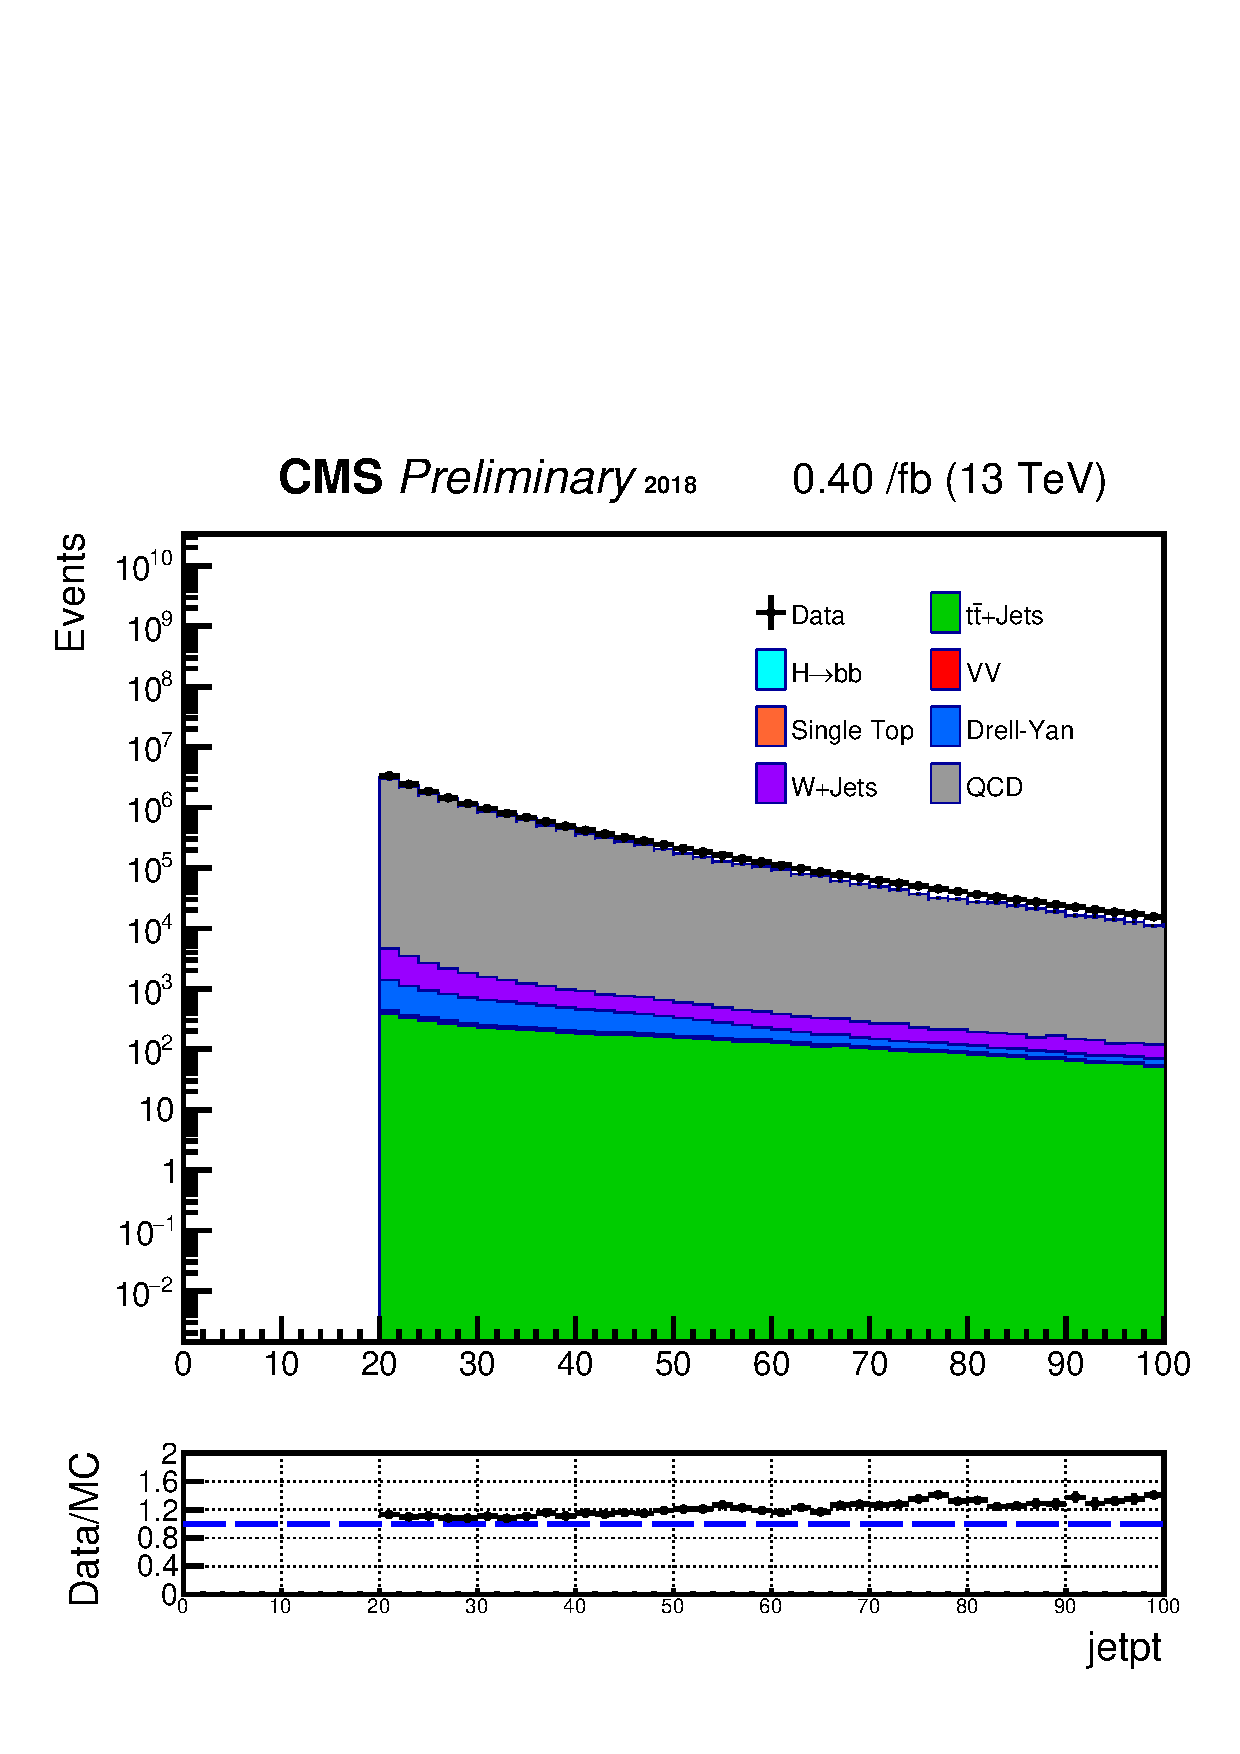
\includegraphics[width=0.47\linewidth]{figs/Data_AnalysisNoteplot_MS-15_ctauS-10_jetpt.pdf}
  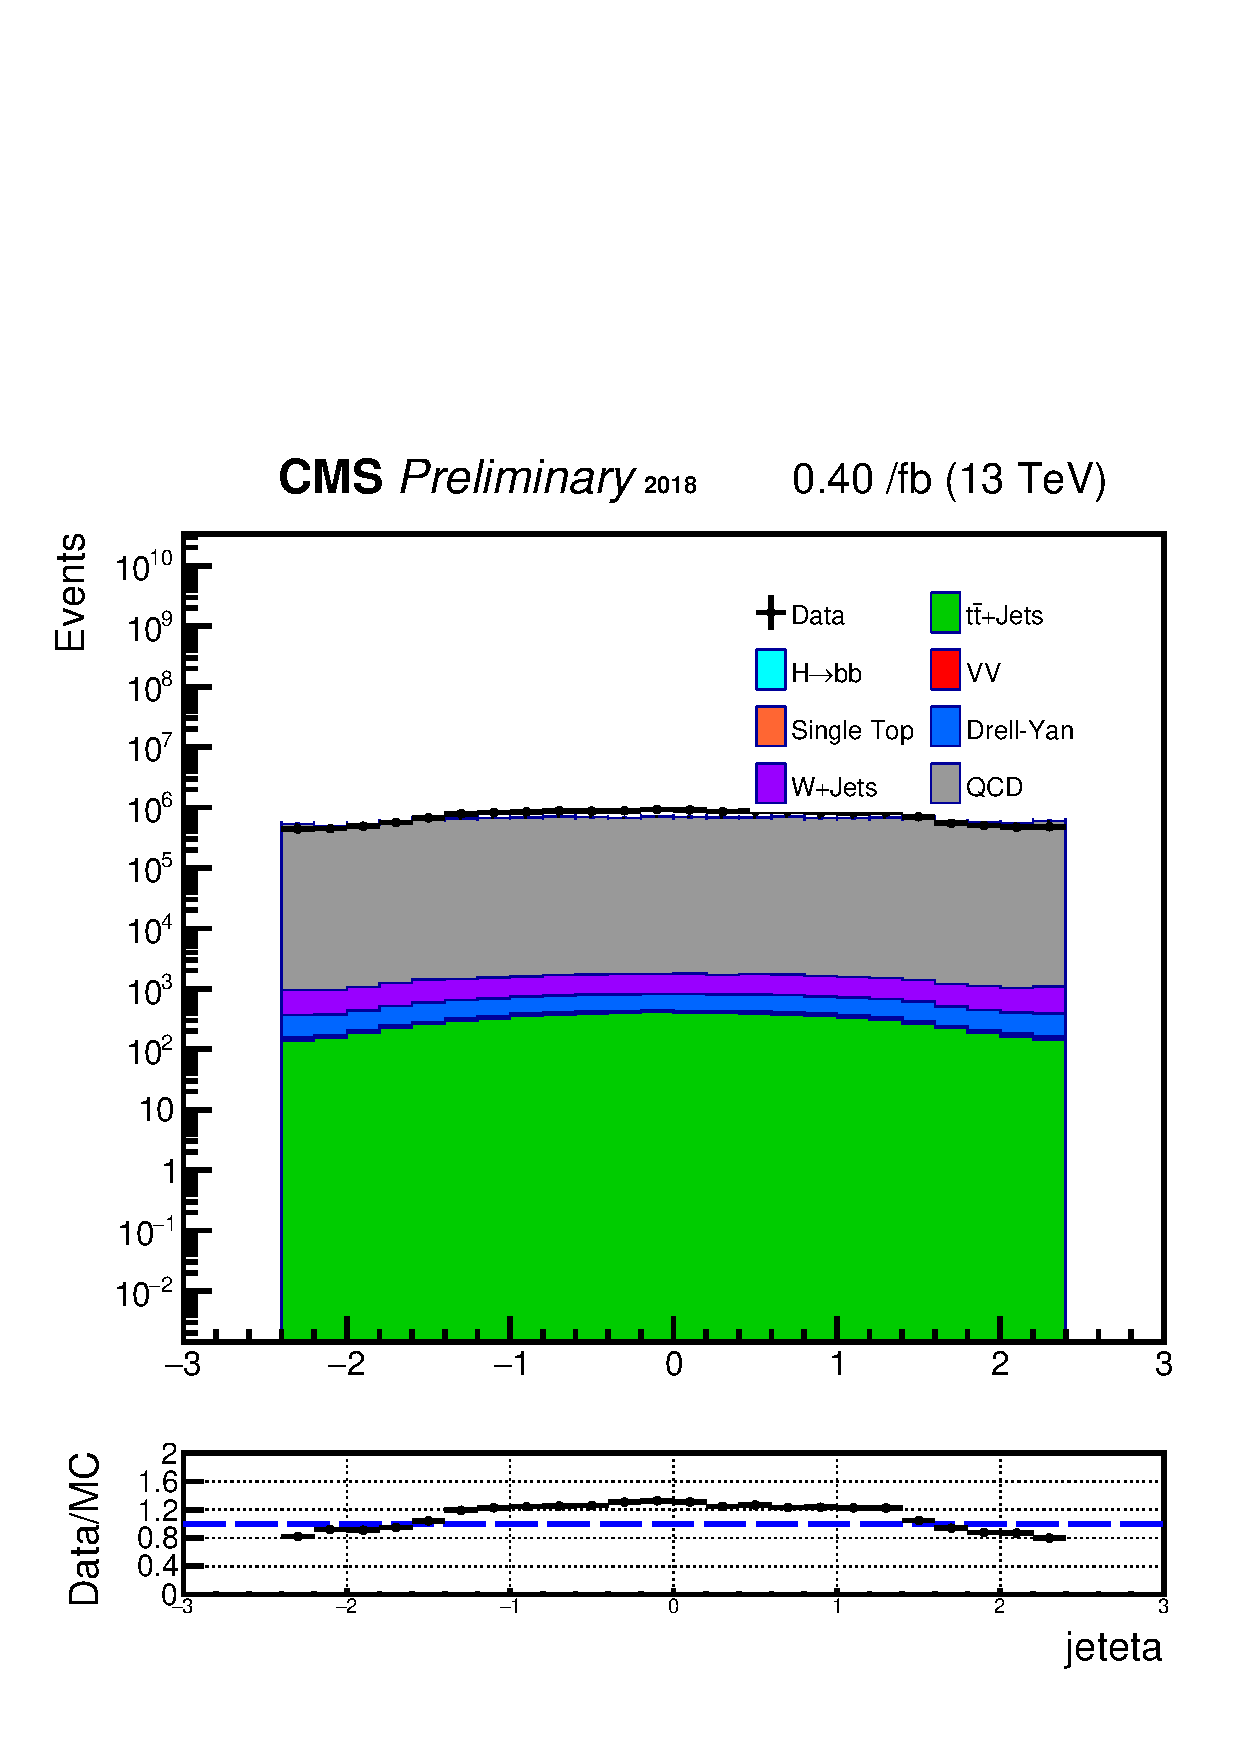
\includegraphics[width=0.47\linewidth]{figs/Data_AnalysisNoteplot_MS-15_ctauS-10_jeteta.pdf}
\end{figure}

\section{Taus}\label{sec:taus}

The analysis sources PAT::slimmedTaus from MINIAOD for MC and RECO::slimmedTaus for Data to produce {\tt selectedTaus}.
$\tau$ leptons have a 64\% branching ratio to hadrons. The Hadron-Plus-Strip (HPS) algorithm enables the reconstruction of a $\tau$ lepton's hadronic decay. 
HPS uses PFJets as its starting point. 
$\tau$'s hadronic decay can be reconstructed with PFJets' charged hadrons in HCAL and 2 $\gamma$s from $\pi^{0}$ decays in ECAL.  
Tau objects require
\begin{itemize}
  \item pt $\geq$ 20 GeV
  \item $|\eta|$ $\leq$ 2.4
\end{itemize}

\begin{figure}[h!]
  \caption{Data/MC of tau objects}
  \label{fig:taus}
  \centering
  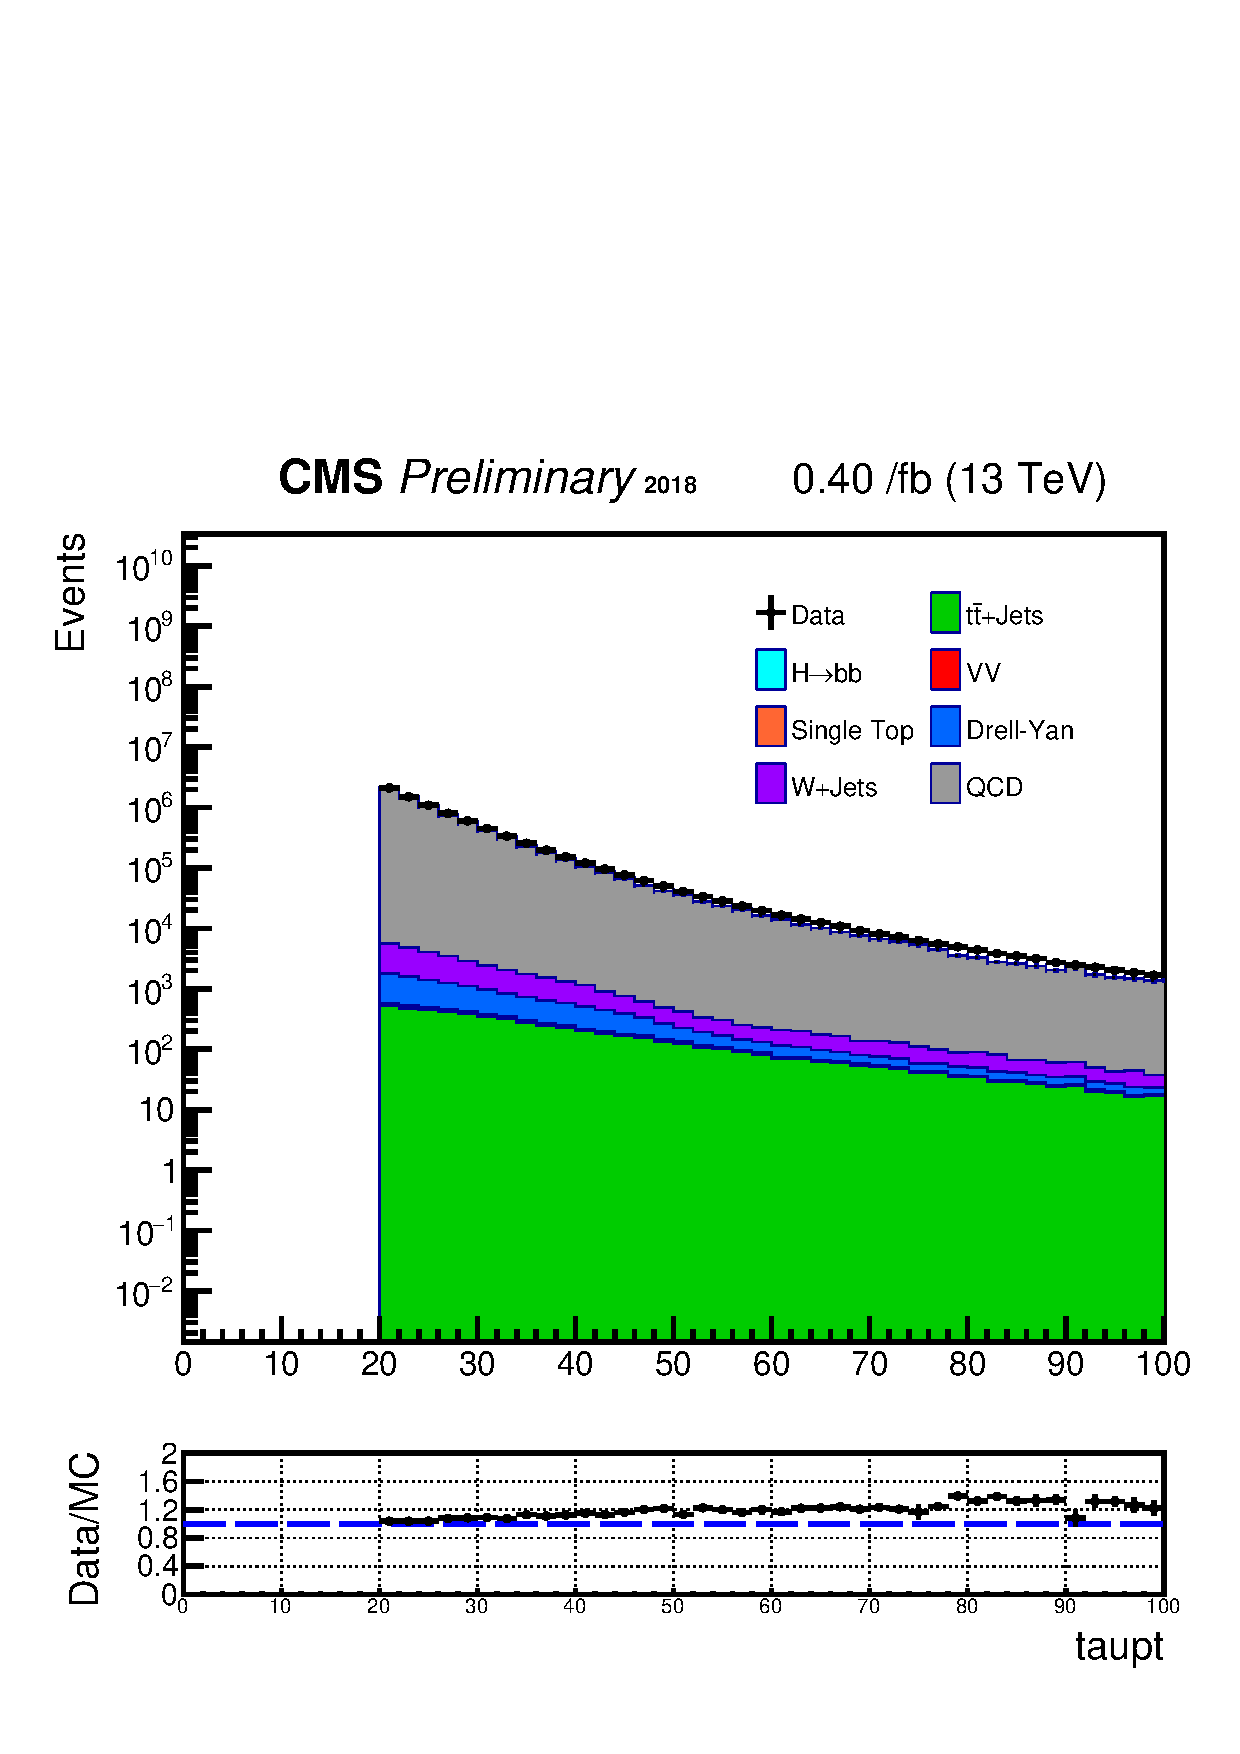
\includegraphics[width=0.47\linewidth]{figs/Data_AnalysisNoteplot_MS-15_ctauS-10_taupt.pdf}
  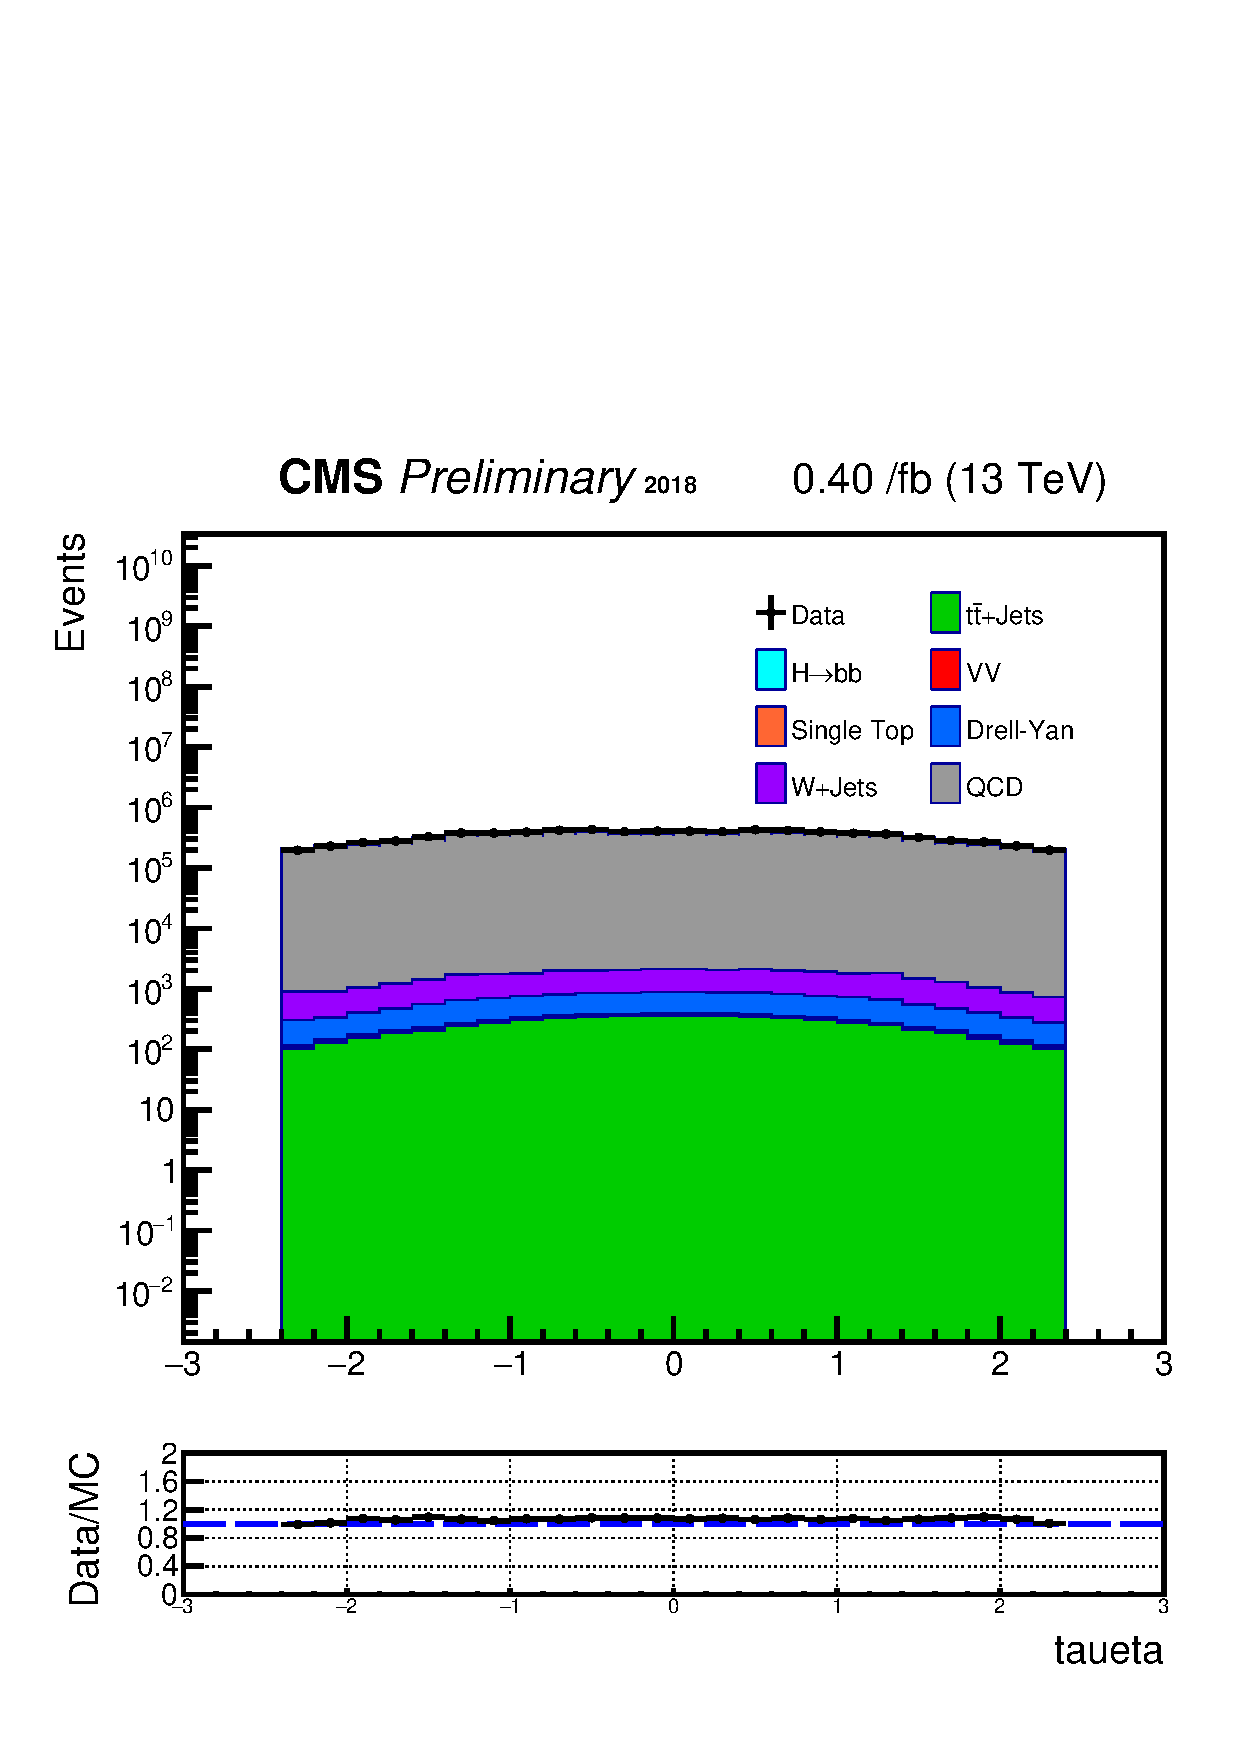
\includegraphics[width=0.47\linewidth]{figs/Data_AnalysisNoteplot_MS-15_ctauS-10_taueta.pdf}
\end{figure}
\section{Region of Interest}\label{sec:ROIs}

The complete reconstruction procedure of Regions of Interest is detailed in the following subsections.
An ROI requires
\begin{itemize}
  \item Good quality track selection
  \item Vertex Fitted from pair-wise tracks by V0Fitter in CMSSW
  \item Cluster the fitted vertices to form a Region of Intrest (ROI)
  \item Look for tracks around $\Delta R=0.3$ around ROI to save its isolation information
\end{itemize}

\subsection{Tracks}\label{sec:ROI_tracks}

The analysis sources packedPFCandidates and lostTracks from MINIAOD.
Track parameters and convariance values will be propagated along the ROI production process and no value should be non-physical
\begin{itemize}
  \item !isinf(tracks.parameter)  and !isnan(tracks.parameter) 
  \item !isinf(tracks.covariance) and !isnan(tracks.covariance) 
  \item Number of valid hits $>$ 3
  \item pt $\geq$ 0.35
  \item Track $IPSig_{XY}\geq$2.
  \item Track $IPSig_{Z}\geq$-1.
  \item Track normalized $\chi^{2}\geq$10.
\end{itemize}


\subsection{Vertex Fitter}\label{sec:ROI_V0Fitter}

The analysis sources offlineBeamspot from MINIAOD for beamspot reference.
Vertex fitter is KalmanVertexFitter with vertex cuts as below.
\begin{itemize}
  \item Vertex $\chi^{2}\geq$6.63 
  \item Transverse Decay distance significance$\geq$15.
  \item V0mass $\geq$13000GeV
  \item cos($\theta_{XY}$) between x and p of V0 candidate $\geq$ 0
  \item cos($\theta_{XYZ}$) between x and p of V0 candidate $\geq$ -2
\end{itemize}


\subsection{ROI formation}\label{sec:ROI_ROIformation}

Fitted vertices are clustered to form a Region of Interest (ROI).
These ROIs have cuts on their parameters as below.
\begin{itemize}
  \item Radius of ROI $\geq$ 1 cm
  \item Annulus $\Delta R \leq$ 0.3 
\end{itemize}

\begin{figure}[h!]
  \caption{Data/MC of ROI distribution}
  \label{fig:ROIs}
  \centering
  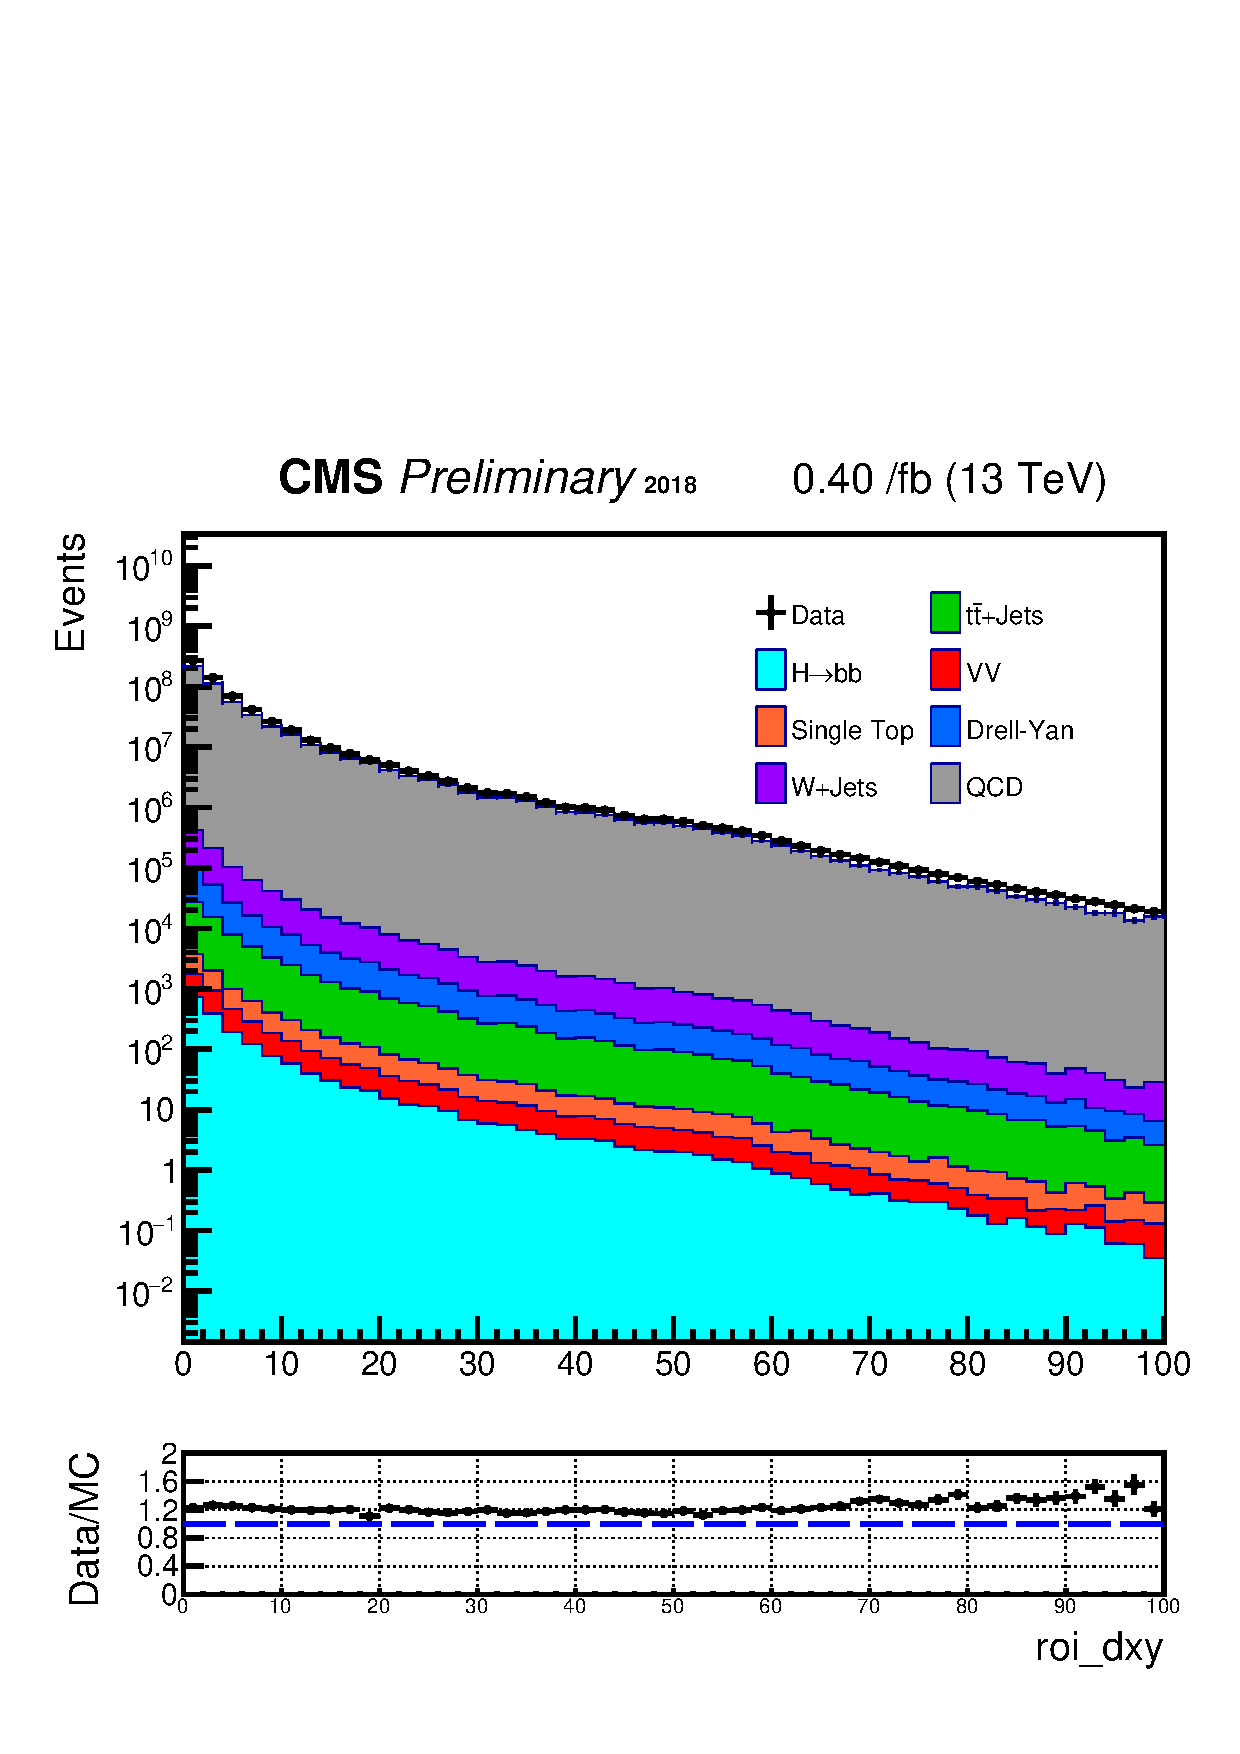
\includegraphics[width=0.47\linewidth]{figs/Data_AnalysisNoteplot_MS-15_ctauS-10_roi_dxy.pdf}
  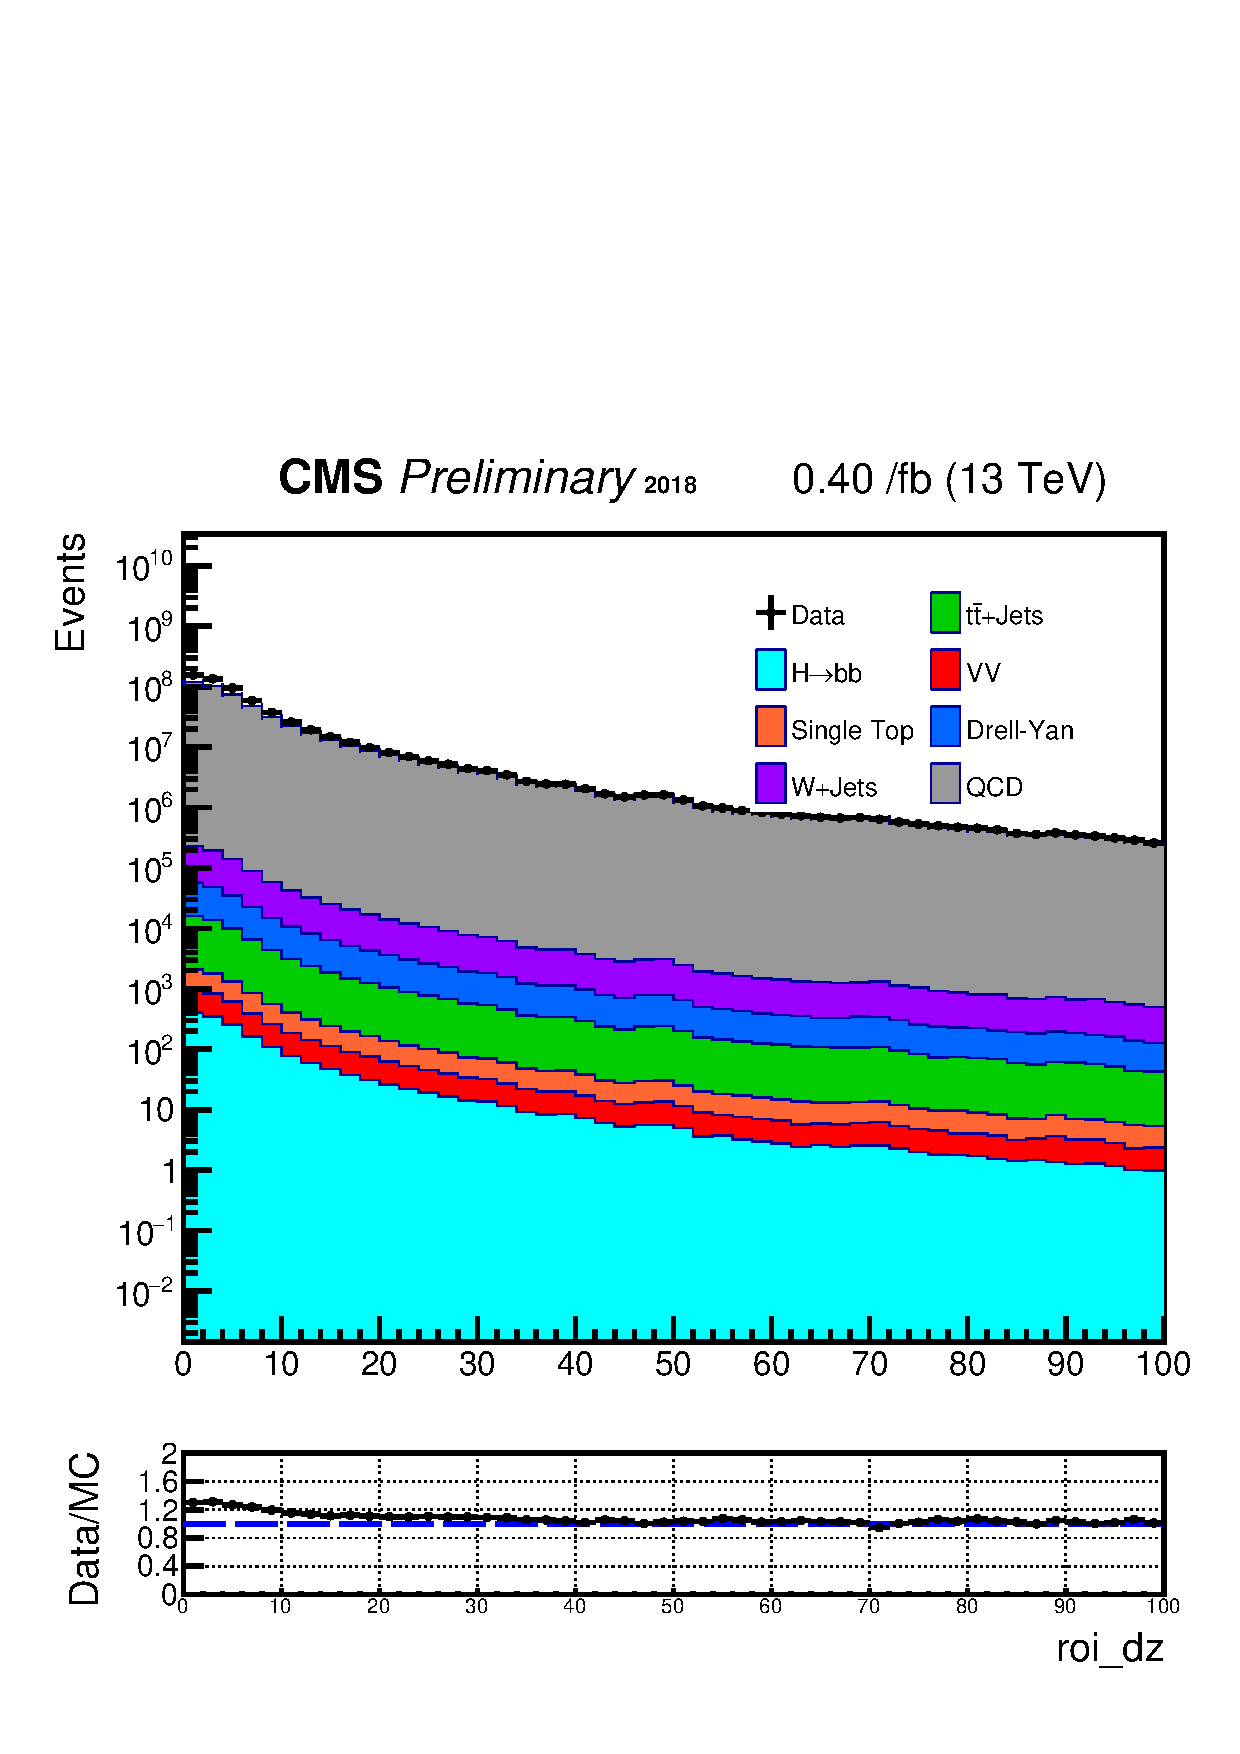
\includegraphics[width=0.47\linewidth]{figs/Data_AnalysisNoteplot_MS-15_ctauS-10_roi_dz.pdf}
\end{figure}

\begin{figure}[h!]
  \caption{2Data/MC of ROI distribution}
  \label{fig:2ROIs}
  \centering
  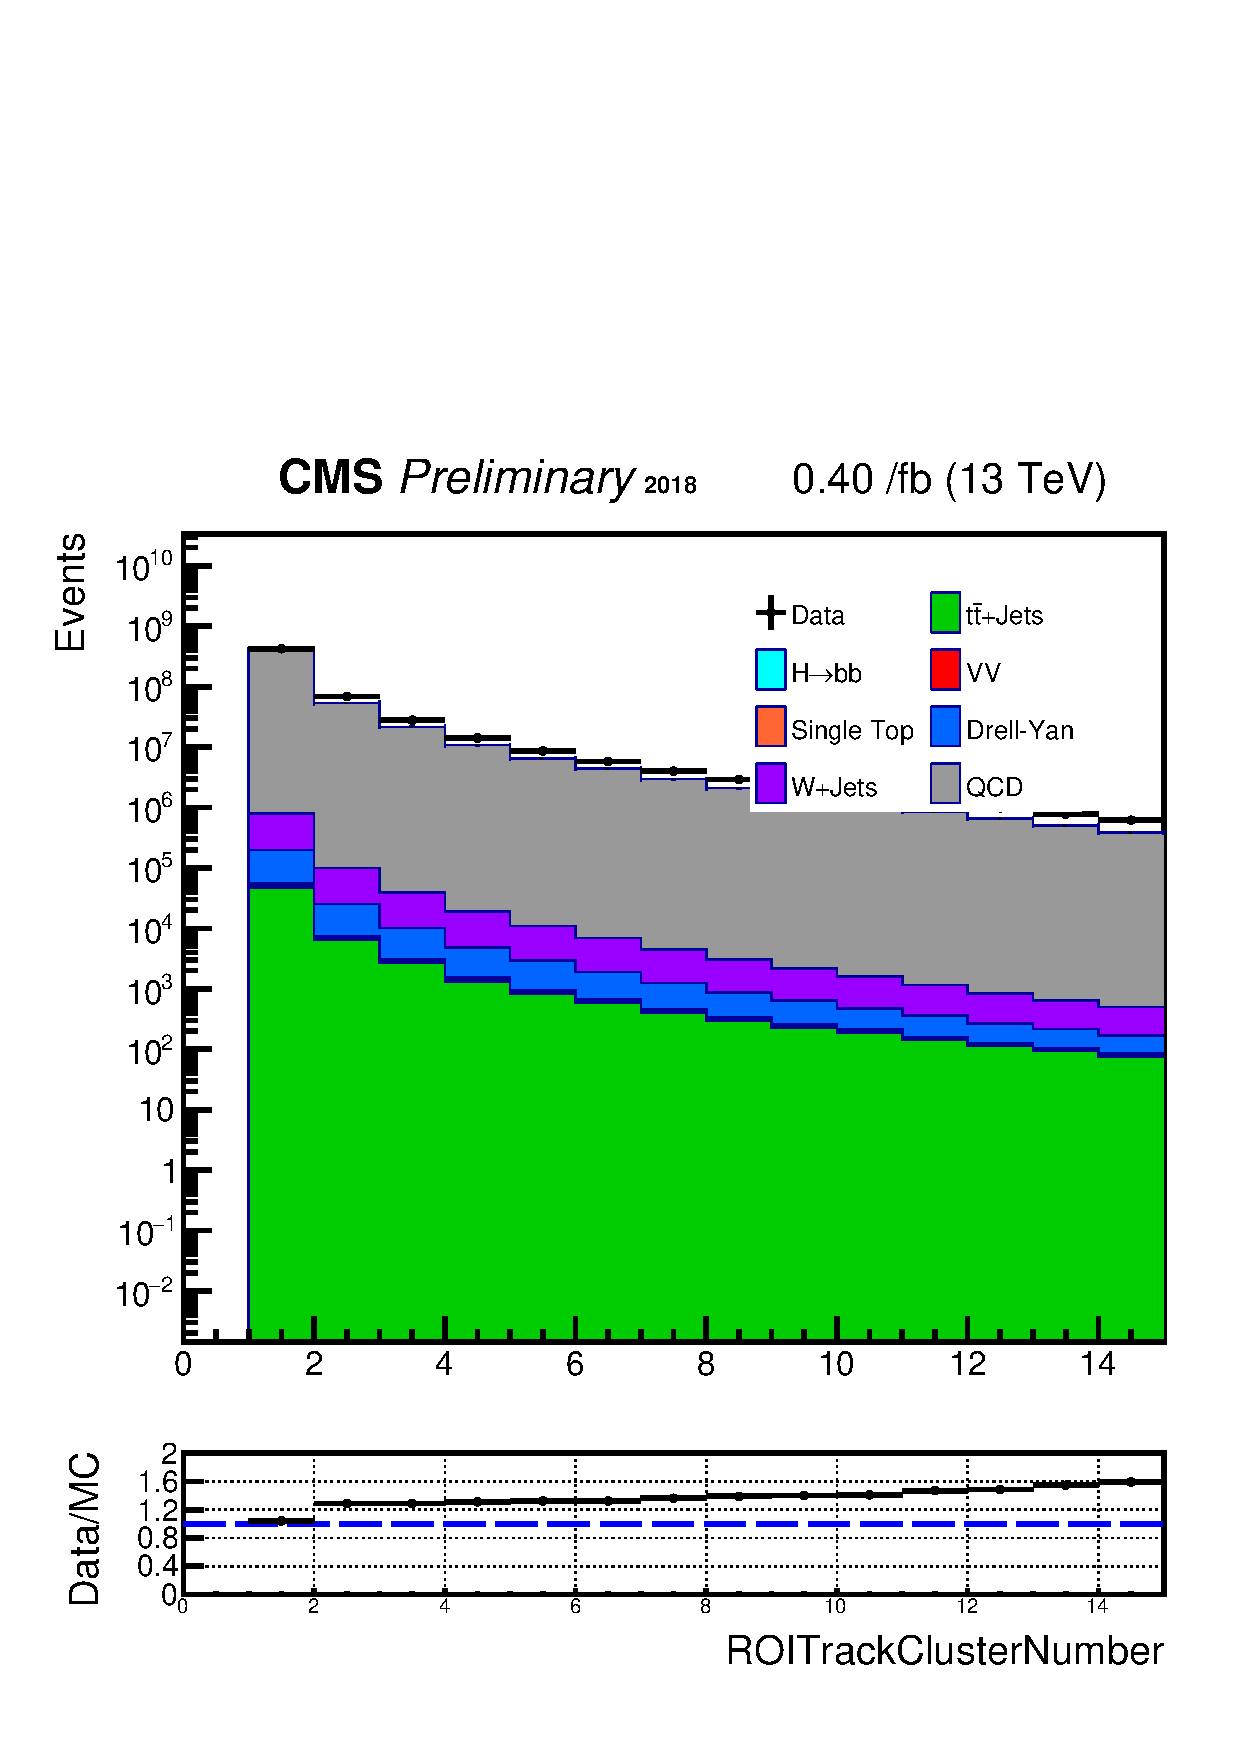
\includegraphics[width=0.47\linewidth]{figs/Data_AnalysisNoteplot_MS-15_ctauS-10_ROITrackClusterNumber.pdf}
  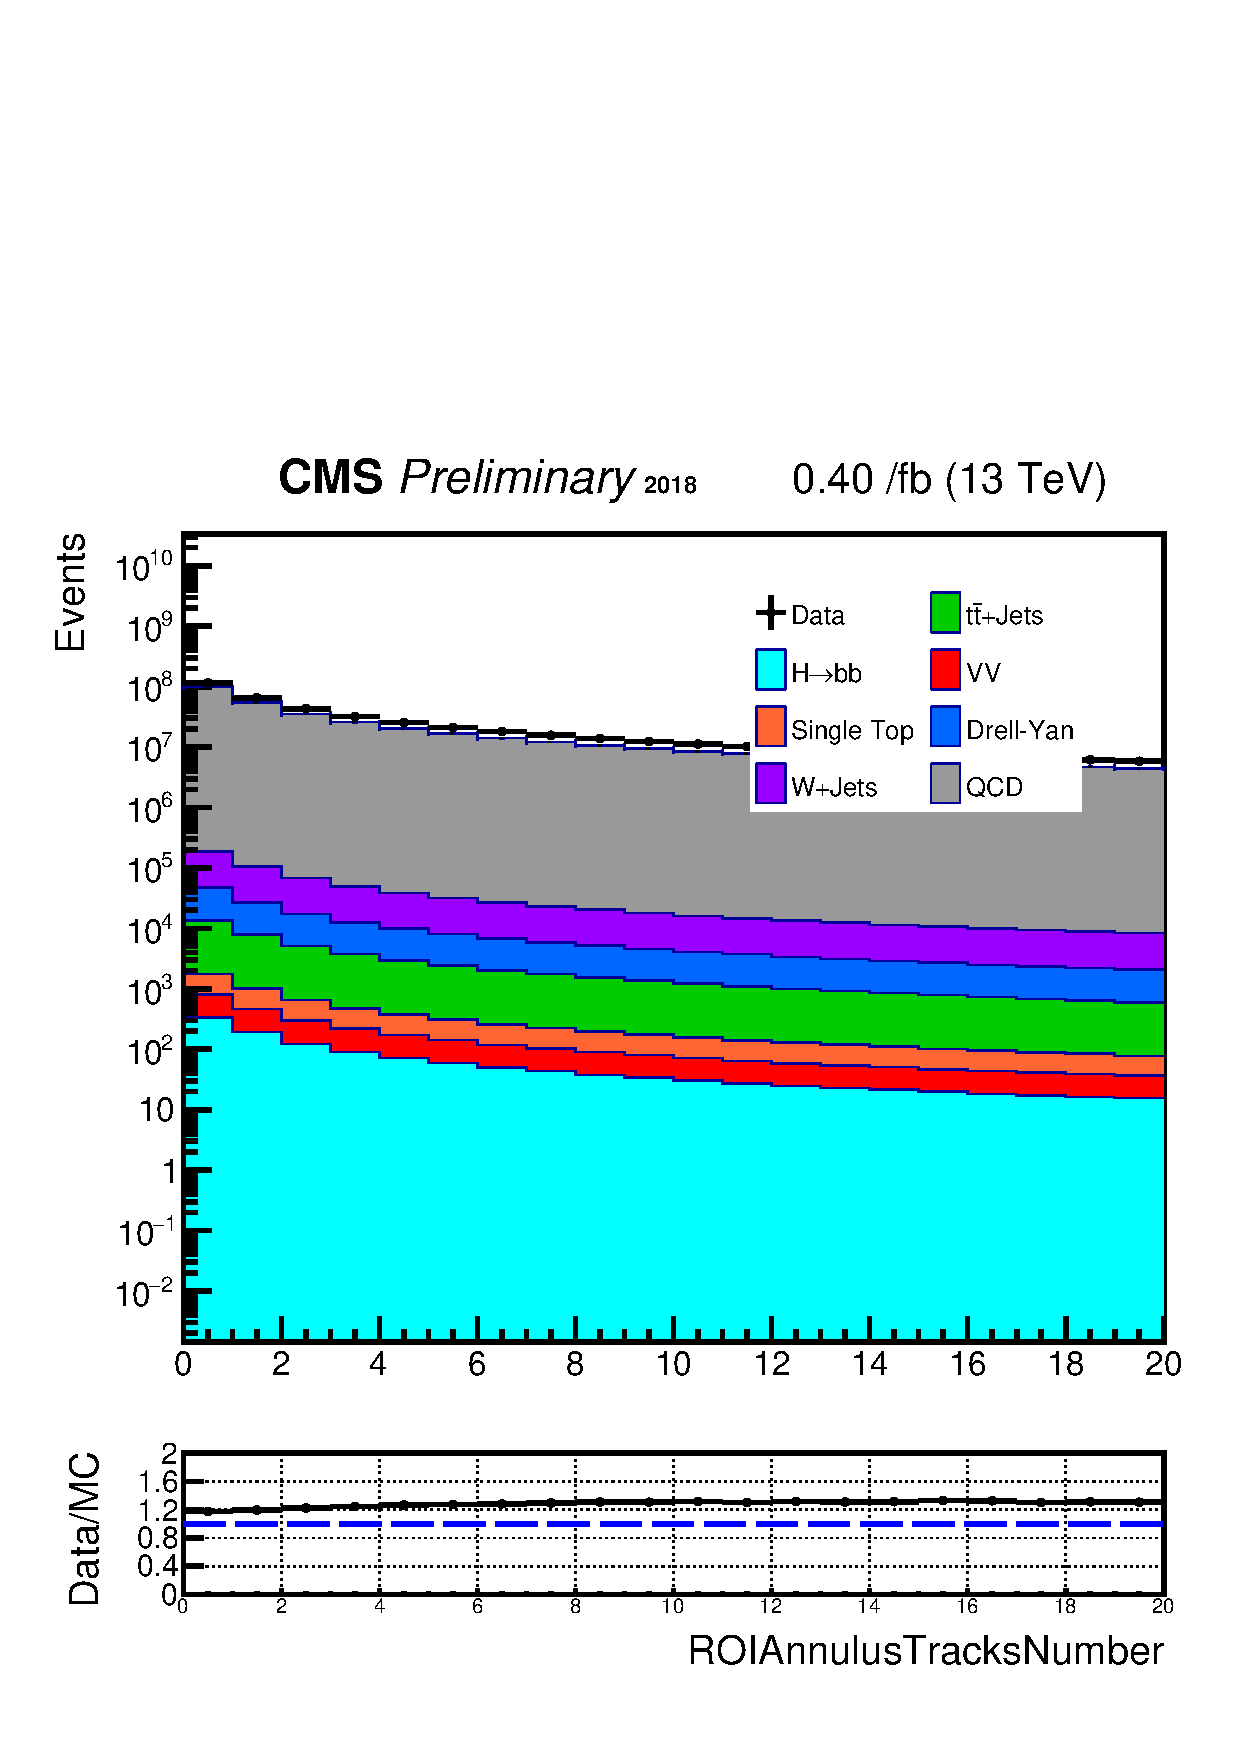
\includegraphics[width=0.47\linewidth]{figs/Data_AnalysisNoteplot_MS-15_ctauS-10_ROIAnnulusTracksNumber.pdf}
\end{figure}
